% =========================================================
% CAPÍTULO II: MARCO TEÓRICO
% =========================================================

\section{Capítulo II - Marco Teórico}

\subsection{Conceptos Operativos y Administrativos}

Se definirán conceptos bases que rigen la operación financiera de la empresa, estableciendo la naturaleza de las cuentas que el sistema propuesto busca optimizar. Por lo que es necesario conocer sobre el área contable, para poder comprender de qué manera esta será aplicada dentro del sistema propuesto. Se define conceptos para conocer acerca de la contabilidad, así como de las ramas que existe y también sus elementos y funciones.

\subsubsection{Contabilidad}

La contabilidad no solamente debe comprenderse como un registro de números, sino como un sistema integral que funciona para transformar los daros sin procesar, en información la cual nos servirá para una correcta toma de decisiones.

"La contabilidad es una técnica que se utiliza para el registro de las operaciones que afectan económicamente a una entidad y que produce sistemática y estructuradamente información financiera" (Guajardo Cantú, 2014, p. 7).

"La contabilidad se define como el arte de registrar, clasificar y resumir de manera significativa, y en términos monetarios, las transacciones y eventos que son, al menos en parte, de carácter financiero" (AICPA, 1961, p. 1).

Es decir que es el modo en cómo se controlan los movimientos monetarios o activos fijos de una empresa o persona, ya sean ingresos o egresos, así como ganancias o gastos, mobiliario y equipo, etc.

En el caso del sistema a implementar este se ve reflejado en los procesos como es la caja chica o los cheques posfechados que no están incluidos dentro del software principal, lo que interrumpe la regulación de datos y aumenta la posibilidad de generar errores al momento de control de estos.

\subsubsection{Objetivos de la Contabilidad}

Es muy importante saber cuáles son los objetivos que tiene la contabilidad y como está influye en las empresas.

Según Meigs et al. (2000), la contabilidad actúa como un vínculo entre las actividades económicas y quienes toman las decisiones. Este proceso implica tres pasos fundamentales: la observación de la actividad económica, el registro de dicha actividad en términos monetarios y la comunicación de la información a través de informes o estados financieros.

\textbf{Control de recursos.} La contabilidad permite que la empresa tenga conocimiento sobre sus ingresos y egresos, como se manejan los activos y a que proveedores se les debe pagar. Según Guajardo Cantú (2014), un objetivo primordial es proporcionar una imagen fiel de la situación financiera de la entidad.

\textbf{Rendición de cuentas.} Ayuda a la empresa para que esta presente resultados de manera correcta y transparente, ante los socios y entidades del estado como lo es la Superintendencia de Administración Tributaria (SAT) en Guatemala.

\textbf{Base para la Planeación.} A través de la contabilidad administrativa, nos podemos anteponer a situaciones que pueden generar perdidas dentro de la empresa, se pueden proyectar también flujos de caja. Para el sistema propuesto busca por medio de las alertas poder cumplir este objetivo para poder anticipar las salidas de efectivo.

\subsubsection{Elementos Básicos de la Contabilidad}

También es necesario conocer los elementos básicos de la contabilidad los cuales comprenden de: Activo, Pasivo, y Capital.

Activo = Pasivo + Capital

\textbf{Activo.} Son los recursos y derechos de la empresa, como lo que pueden ser el ingreso monetario. En el sistema propuesto se identificarán como el ingreso monetario por medio de los cheques que envían los clientes y el efectivo que se maneja por medio de la caja chica, los cuales requieren de un control extremadamente estricto, para poder evitar pérdidas. "Un activo es un recurso económico propiedad de una entidad, que se espera rinda beneficios en el futuro" (Guajardo Cantú, 2014, p. 50).

\textbf{Pasivo.} Son las obligaciones y deudas que se tienen hacia terceros, también conocido como el gasto monetario. Para el sistema propuesto este se logra identificar por medio de las facturas que emiten los proveedores las cuales debemos registrar para realizar los pagos a futuro, también corresponde al momento de reintegrar viáticos a los colaboradores de la empresa. "El pasivo representa lo que el negocio debe a otras personas o entidades conocidas como acreedores" (Guajardo Cantú, 2014, p. 51).

\textbf{Capital.} Son las diferencias que se tienen entre activo y pasivo, es decir representa el valor residual de los accionistas de la empresa. "El capital es la parte de los activos que pertenece a los dueños del negocio" (Horngren et al., 2012, p. 12).

\subsubsection{Ramas o Especializaciones de la Contabilidad}

Ahora bien, ya se conoce los elementos básicos de la contabilidad. Entonces procedemos a definir como es que la contabilidad está dividida o ramificada, esto sucedió ya que la contabilidad se tuvo que obligar a evolucionar para poder satisfacer las necesidades de diversos usuarios. Según esta doctrina contable, estas ramas permiten que las empresas, no solamente cumpla con la ley, sino que también puedan optimizar los recursos internos, tanto monetarios como mobiliarios entre otros.

\textbf{Contabilidad Financiera.} Esta rama está centrada principalmente en la preparación de estados financieros para usuario externos los cuales podría ser como inversionistas, entidades bancarias y organismos reguladores en Guatemala. Se rige por reglas estrictas. En Guatemala estas suelen basarse en las Normas Internacionales de Información Financiera (NIIF).

"La contabilidad financiera se concentra en la elaboración de estados financieros que son de utilidad para agentes externos y para la gerencia, proporcionando un registro histórico de los recursos y obligaciones de la entidad" (Meigs et al., 2000, p. 5).

"El propósito de la contabilidad financiera es proporcionar información que sea útil para los inversionistas y acreedores actuales y potenciales al tomar decisiones racionales" (Horngren et al., 2012, p. 4).

Esta rama es en la que se concentra principalmente el software que se encuentra implementado en la empresa, ya que asegura que los balances cuadren legalmente, por lo que al ser más para factores externos, no está muy centrado en el área interna y acá es donde se desea complementar por medio del sistema propuesto.

\textbf{Contabilidad Administrativa.} Esta rama se diferencia de la contabilidad financiera, quien recopila información del pasado y lo presenta de esa forma, en cambio en la contabilidad administrativa trata de predecir el futuro, centrándose en la probabilidad de que algo pueda ocurrir.

"La contabilidad administrativa se enfoca en el futuro y proporciona información para la planeación y el control de las operaciones de la organización" (Meigs et al., 2000, p. 6).

"Se enfoca en las necesidades de los usuarios internos y no está sujeta a los principios de contabilidad generalmente aceptados" (Horngren et al., 2012, p. 5).

Para la empresa esta rama es vital porque permite gestionar el ``día a día''. El control de pago a proveedores, por ejemplo, no solo es un registro de un gasto, sino una herramienta que advierte que dicho gasto se realizara en tal fecha por lo que se debe contemplar que en esa fecha exista dicho fondo para poder ser desembolsado.

\textbf{Contabilidad Fiscal.} Esta rama esta especializada fundamentalmente en las leyes tributarias. El objetivo principal es asegurar que la empresa determine y pague correctamente sus impuestos, como, por ejemplo, el Impuesto al Valor Agregado (IVA) y el Impuesto Sobre la Renta (ISR).

La contabilidad fiscal se refiere a la preparación de los informes de impuestos y el cumplimiento con las leyes tributarias respectivas" (Guajardo Cantú, 2014, p. 15).

En el sistema propuesto utilizara esta rama para poder gestionar dichos impuestos y que estos sean debidamente calculados y poderlos incluir dentro del software de la empresa.

\textbf{Contabilidad de Costos.} Esta rama se puede decir que está ligada a los inventarios. Se encarga de clasificar, acumular y asignar valores para determinar cuánto cuesta producir un bien o prestar algún servicio. En la empresa se representa en el análisis de los gastos asociados a la adquisición y distribución de los productos farmacéuticos, permitiendo medir la eficiencia en el uso de los recursos y establecer precios de venta competitiva.

\begin{table}[h]
    \centering
    \caption{Comparativa entre Contabilidad Financiera y Administrativa}
    \vspace{0.2cm}
    \begin{tabular}{p{3cm} p{5cm} p{5cm}}
        \toprule
        \textbf{Característica} & \textbf{Contabilidad Financiera} & \textbf{Contabilidad Administrativa} \\
        \midrule
        Usuarios & Externos (Bancos, SAT) & Internos (Gerencia, Contador) \\
        Normativa & Obligatoria (NIIF/PCGA) & Opcional (Según necesidad) \\
        Enfoque & Histórico (Pasado) & Prospectivo (Futuro/Alertas) \\
        Sistema en la empresa & software & Aplicación Web propuesta \\
        \bottomrule
    \end{tabular}
    
    \vspace{0.2cm}
    \raggedright \small \textbf{Nota.} \textit{Elaboración propia basada en Meigs et al. (2000) y tipos de contabilidad.}
\end{table}

Se puede ver en la Tabla 1 una pequeña comparativa entre la Contabilidad que Maneja la empresa por medio del Software y la Contabilidad que el sistema propuesto desea cubrir.

\subsubsection{Fundamentos del Control Interno}

Como se vio anteriormente el sistema propuesto utilizara en su mayor parte la contabilidad Administrativa, por lo que ahora se hablara sobre el Control Interno y como las empresas o utilizan para proteger sus activos y asegurar la exactitud de sus registros contables.

El control interno se define como el conjunto de políticas y procedimientos diseñados para proporcionar una seguridad razonable en cuanto al logo de los objetivos de la entidad. En una organización, cuya operación involucra el manejo de suministros médicos y flujos constantes de efectivo, el control interno es la herramienta que garantiza la integridad de la información financiera.

De acuerdo con Meigs et al. (2000, p. 152), un sistema de control interno sólido tiene cuatro objetivos principales: proteger los activos contra el robo o desperdicio, asegurar la exactitud y confiabilidad de los registros contables, promover la eficiencia operativa y estimular el cumplimiento de las políticas administrativas. En la actualidad, la dependencia de procesos manuales y hojas de cálculo para el control de documentos contables complementarios representa un riesgo para el cumplimiento de estos objetivos.

El sistema propuesto utilizara el control interno para el asegurar que el manejo de los activos sean de manera confiable y segura, por ejemplo, en el pago de viáticos el control interno se aplicaría al momento de registrar a que personas se les debe reintegrar viáticos en la semana y que personas se le reintegra la próxima, Se deja en claro las personas que utilizan los viáticos y las personas que se quedan en espera, también se queda en registro el monto de reintegro y a que pertenece, (comida, depreciación, combustible o parqueo), todos estos control también pueden servir para una proyección a futuro de que gastos se realiza el colaborador más seguido.

\textbf{El ambiente de Control y Gestión de Riesgos.} "El ambiente de control es la base de todos los demás componentes del control interno; proporciona disciplina y estructura" (Guajardo Cantú, 2014, p. 212), este refleja la actitud global de la administración hacia la importancia del control en la organización. La identificación de errores operativos, como el retraso en el pago a proveedores por fallas en calendarios físicos, evidencia la necesidad de fortalecer este ambiente mediante soluciones tecnológicas.

"Las actividades de control incluyen una gama de actividades tan diversas como aprobaciones, autorizaciones, verificaciones y conciliaciones" (Estupiñán Gaitán, 2015, p. 32).

Por otro lado, la evaluación de riesgos consiste en identificar y analizar los factores que podrían impedir que la empresa logre sus metas. En el área contable, no se puede permitir tener el riesgo de pérdida de información por eso se determina que el uso excesivo de archivos de Excel (hasta diez archivos mensuales) es un factor critico que el sistema propuesto desea mitigar. Al tener todo unificado y en su mayoría automatizado, podemos reducir este riesgo de pérdida de información, ahorrarnos memoria y reducir el tiempo de labor que se empeña realizando estas tareas monótonas.

Para profundizar en la seguridad de la información, es necesario citar a Estupiñán Gaitán (2015), quien define el control interno no solo como un conjunto de manuales, sino como un proceso efectuado por el personal de una entidad, diseñado para enfrentar los riesgos que amenazan el cumplimiento de los objetivos.

\begin{table}[h]
    \centering
    \caption{Matriz de Riesgos y Controles Propuestos}
    \vspace{0.2cm}
    \begin{tabular}{p{3cm} p{5cm} p{5cm}}
        \toprule
        \textbf{Proceso} & \textbf{Riesgo Identificado} & \textbf{Control Sugerido (Sistema Web)} \\
        \midrule
        Pago a proveedores & Pagos fuera de tiempo por errores manuales & Sistema de alertas automáticas parametrizadas \\
        Gestión de caja chica & Pérdida de documentos de respaldo físico & Repositorio digital centralizado en PostgreSQL \\
        Control de archivos & Saturación de memoria y archivos anticuados & Base de datos escalable en la nube \\
        Cálculos de fechas & Errores en la consideración de feriados & Algoritmos de cálculo automático en Python \\
        \bottomrule
    \end{tabular}
    
    \vspace{0.2cm}
    \raggedright \small \textbf{Nota.} \textit{Elaboración propia basada en Meigs et al. (2000) y el planteamiento del problema identificado.}
\end{table}

También nos dice que el control interno se divide en componentes clave:

\textbf{\textit{Información y Comunicación.}} Se refiere a poder identificar y capturar la información de tal forma que permita a los empleados cumplir con sus responsabilidades en un periodo de tiempo razonable. El uso de archivos en Excel puede impedir que esta comunicación sea efectiva y de manera fluida entre el contador y administrado.

\textbf{\textit{Actividades de Control.}} Son normas y políticas internas de la empresa, normalmente indicadas por gerencia, para asegurar la efectividad de manejo de los activos y pasivos de la empresa. Al momento de implementar el sistema de alertas automáticas para cheques posfechados y pagos a proveedores, es considerada una actividad de control preventivo que promueve a cumplir con las normas y políticas establecidas, como, por ejemplo, que los cheques se depositen un día después de fecha, si esta corresponde a un feriado o fin de semana, esto reduce la probabilidad de que el cheque se deposite en un rango fuera de la fecha del depósito.

Las actividades de control son las políticas que ayudan a asegurar que se tomen las medidas necesarias para orientar los riesgos hacia el logro de los objetivos. Horngren et al. (2012) destaca que las verificaciones independientes y la documentación adecuada son esenciales para un control efectivo.

\begin{table}[h]
    \centering
    \caption{Componentes del Control Interno aplicados al Proyecto}
    \vspace{0.2cm}
    \begin{tabular}{p{3cm} p{5cm} p{5cm}}
        \toprule
        \textbf{Componente} & \textbf{Aplicación Técnica en el Sistema} & \textbf{Objetivo de Mejora} \\
        \midrule
        Información & Centralización de documentos de respaldo & Eliminar la dispersión de datos en Excel \\
        Comunicación & Notificaciones oportunas de pagos y depósitos & Optimizar la visualización de fechas clave \\
        Supervisión & Acceso a reportes para auditoría interna & Facilitar la fiscalización de procesos \\
        \bottomrule
    \end{tabular}
    
    \vspace{0.2cm}
    \raggedright \small \textbf{Nota.} \textit{Adaptado de Meigs et al. (2000) y Horngren et al. (2012).}
\end{table}

\subsubsection{El Ciclo Contable y la Documentación de Respaldo}

Se define como el proceso ordenado y detallado de pasos que permiten transformar una transacción económica en un registro financiero formal. "El ciclo contable es el proceso repetitivo de pasos que permite transformar una transacción económica en un registro financiero formal" (Meigs et al., 2000, p. 110).

Sin embargo, para que este ciclo sea válido es necesario tener documentación de respaldo la cual debe estar de acuerdo con la ley, que es gestionada por medio de SAT, Guajardo Cantú (2014, p. 212) enfatiza que "la confiabilidad de la información contable depende de la existencia de documentos fuente que respalden la validez de cada entrada en el diario". En la empresa donde se desplegará el sistema propuesto, este respaldo es crítico debido al registro que consisten en importaciones o gastos de viáticos entre otros, estos documentos deben estar perfectamente vinculadas con el registro digital. Actualmente solo algunos registros se llevan dentro del software de la empresa y esta es otra de las problemáticas que el sistema propuesto desea resolver, poder dejar registro de estos documentos de respaldo. Por parte de las entidades de gobierno como lo es SAT nos establece que, en el {Decreto 10-2012 (Ley de Actualización Tributaria)}, establece que los gastos solo serán deducibles si corresponden a operaciones necesarias para producir renta y están documentados legalmente.

\begin{table}[h]
    \centering
    \caption{Ejemplos de Documentación de respaldo}
    \vspace{0.2cm}
    \begin{tabular}{p{3.5cm} p{3.5cm} p{6cm}}
        \toprule
        \textbf{Tipo de movimiento} & \textbf{Función Contable} & \textbf{Control de Documentos de Respaldo} \\
        \midrule
        Proveedores & Gasto operativo & Facturas con respaldo SAT \\
        Caja Chica & Gasto Menor & Vales de desembolso de efectivo, facturas que respaldan la compra. \\
        Clientes & Ingreso & Cheques de clientes con fechas específicas para deposito \\
        Colaboradores & Gasto Operativo & Facturas para reintegro de viáticos \\
        \bottomrule
    \end{tabular}
\end{table}

La tabla 4 muestra un breve ejemplo de los documentos de respaldo que utilizaremos como base para el sistema propuesto, Podemos observar el que el tipo de movimiento corresponde de donde se obtiene documento, si es por medio de un proveedor, es relacionado a caja chica, es por medio de un cliente o por los colaboradores. La función contable define como es que interactúa estos documentos en relación financiera, es decir como se identifica el gasto o el ingreso monetario. El ingreso monetario hace mención al tipo de documento o la verificación de estos, por ejemplo, si es una Factura, esta debe estar avalada por la SAT, si es un Vale este debe contener la firma del contador y sello si es corresponde, etc.

\begin{figure}[h]
    \caption{Ejemplo de Factura Electrónica (FEL)}
    \vspace{0.2cm}
    \centering
    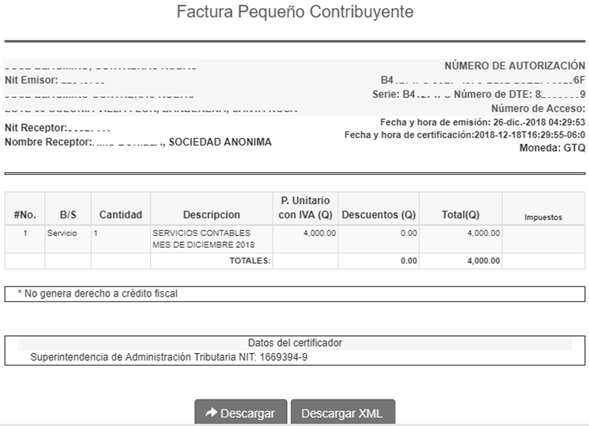
\includegraphics[width=0.8\textwidth]{imagenes/image2.png}
    
    \vspace{0.2cm}
    \raggedright \small \textbf{Nota.} \textit{Figura obtenida de \url{https://preguntas.diamantecontador.com}}
\end{figure}

En la figura 1 podemos apreciar una factura por medio del portal SAT este documento de respaldo es admitido en la Empresa, para hacer validación de Facturas de Proveedores, Facturas para viáticos y Facturas para liquidación de caja chica.

En el caso de la caja chica, se entrega primeramente un vale de caja chica, para poder desembolsar el efectivo y luego la persona que recibió el efectivo, deberá entregar un documento de respaldo como lo es la Factura contable, que debe tener el mismo monto del vale o bien debe reembolsar la diferencia entre el gasto y el efectivo entregado.

\begin{figure}[h]
    \caption{Ejemplo de Vale de Caja chica}
    \vspace{0.2cm}
    \centering
    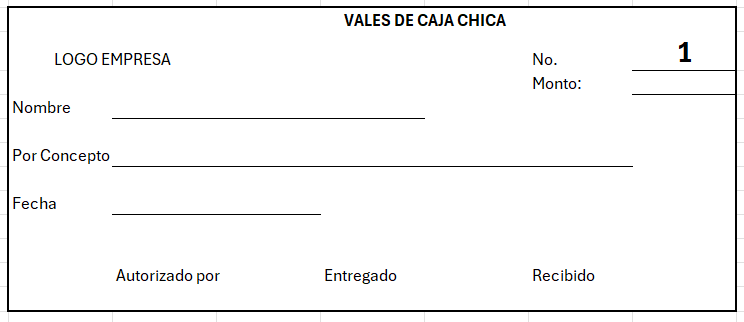
\includegraphics[width=0.8\textwidth]{imagenes/image3.png}
\end{figure}

\begin{figure}[h]
    \caption{Ejemplo de Cheque}
    \vspace{0.2cm}
    \centering
    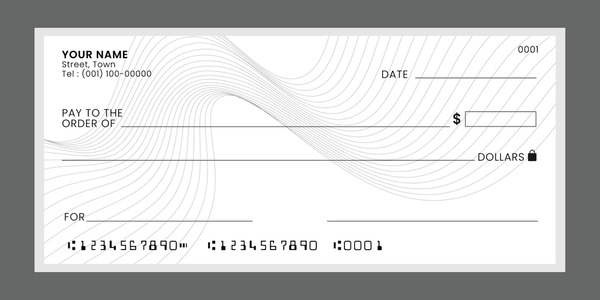
\includegraphics[width=0.8\textwidth]{imagenes/image4.jpeg}
    
    \vspace{0.2cm}
    \raggedright \small \textbf{Nota.} \textit{Figura obtenida de: \url{https://www.shutterstock.com/es/search/chequed}}
\end{figure}

\subsubsection{Gestión de Operaciones de Tesorería y Ciclo de Pagos}

Una Empresa se puede clasificar como buena organización por la forma en como administra sus ingresos y egresos monetarios. En el caso de la empresa en donde vamos a desplegar el sistema propuesto se enfoca en cuatro pilares principales los cuales gestionan el manejo monetario, que requiere de un riguroso control para evitar fugas de capital y errores administrativos.

\textbf{Fondo Fijo de Caja Chica.} Se refiere al fondo disponible que tiene la empresa para cubrir gastos menores, que normalmente no requieren de transferencias o cheques, El manejo de la caja chica es por medio de efectivo.

"El fondo de caja chica es una cantidad fija de efectivo que se utiliza para pagar gastos de pequeña cuantía. El sistema de control requiere que cada pago esté respaldado por un comprobante pre-numerado" (Horngren et al., 2012, p. 248).

Su sistema o control consta de la realización de un vale de caja chica que funge como un documento de respaldo, indicando que se realizó un desembolso de efectivo, pero este documento es provisional. El documento de respaldo de mayor interés corresponde a la factura o recibo que hace constar que se realizo el gasto del efectivo. También hay que tomar en cuenta que no siempre se gasta el efectivo indicado dentro del vale, por lo que es necesario colocar dentro de las observaciones del vale que, al momento de realizar el gasto, este fue menor al previsto, y se debe reintegrar la diferencia del gasto hacia caja chica, por ello se indica que el vale de caja chica solamente es provisional.

El sistema propuesto, permitirá el registro digital de estos comprobantes, facilitando el arqueo de caja chica y la solicitud de reintegro al contador de forma inmediata. Esto se refiere al momento de agotar el efectivo disponible.

\textbf{Gestión de Viáticos y Gastos de Viaje.} Los viáticos comprenden a la asignación de fondo para gastos de lo que los empleados tienen como beneficios. Normalmente los viáticos sirven para cubrir gastos como lo son: Gasolina, Alimentación, Hospedaje, Depreciación (Se refiere a servicio de vehículo o reparación de este).

"Los gastos de viaje deben ser estrictamente controlados mediante informes de gastos que detallen el propósito del viaje y estén acompañados por las facturas originales de soporte" (Estupiñán Gaitán, 2015, p. 55). Este Fondo debe ser fijo y al momento de ser entregados los gastos por viáticos, el empleado no debe exceder el gasto del fondo, es decir, por ejemplo, si al momento de la contratación tiene un desembolso de Q500.00 los cuales corresponden para gastos de alimentos durante 1 semana de viaje, al momento de que el empleado entregue al contador los documentos de respaldo (Facturas), estos deben sumar Q500.00 o un monto menor a ello. Esto es debido a que el contador al momento de realizar el reintegro de estos gastos lo hará al monto del fondo en su caso y si de casualidad si es de monto menor, este se realizara al monto entregado.

En el sistema propuesto, la liquidación de viáticos dejara de ser un proceso en papel o en Excel, dejando también de ser un proceso de calculo manual a realizarse de manera automática, registrando las facturas que la personal entrega. El contador realiza los reintegros generando hojas de Excel por cada reintegro y de manera manual realiza los cálculos. En el sistema propuesto, el contador registrara las facturas únicamente y el sistema generara las partidas automáticamente para que el contador únicamente realice los reintegros correspondientes.

\textbf{Cheques y Títulos de Crédito.} El cheque es un documento mercantil por el que una persona puede realizar transferencias o pagos monetarios hacia otra persona, esto se realiza mediante una entidad bancaria que funciona como intermediario entre la persona A hacia la persona B.

"El control del efectivo requiere que todos los desembolsos importantes se realicen mediante cheque, lo cual proporciona un registro permanente de cada pago" (Meigs et al., 2000, p. 160). Es decir que, a diferencia de la caja chica, los cheques pueden desembolsar cantidades grandes de dinero, son usualmente utilizado para realizar pagos a proveedores o realizar compras de grandes magnitudes. Los cheques también funcionan como documento de respaldo, ya que deja un registro de cuando y cuanto se desembolsó el recurso monetario y también a quien se realizó dicho desembolso.

La empresa lo toma de la parte de recepción de dichos cheques, al ser posfechados, estos tienen indicada una fecha de depósito y son recibidos por el contador quien se debe encargar de depositarlos correctamente en la fecha indicada del cheque, pero en el caso de tener la fecha de depósito en algún día de descanso, es recomendable realizarlo al siguiente día laboral. Este tipo de control es realizado de forma manual por medio de calendarios físicos, careciendo de alertas, por ello el sistema propuesto, promueve el uso de alertas que dan aviso el día correspondiente de depósito y también deja un registro de estos cheques para consultas futuras.

\textbf{Pago a Proveedores y Crédito Comercial.} También conocida como cuenta por pagar. Esta función corresponde a la gestión y control de pagos a proveedores los cuales normalmente contienen días Crédito (lapso que da el proveedor para poder pagar su factura), estos pagos pueden ser por compras de suministros, pago de importaciones, pago por servicios (agua, luz, teléfono etc.), entre otros rublos.

"Las cuentas por pagar representan pasivos a corto plazo que deben gestionarse para aprovechar descuentos por pronto pago y mantener relaciones sólidas con los proveedores" (Guajardo Cantú, 2014, p. 340). Estos beneficios son establecidos al momento de crear la relación empresarial por medio de un contrato entre ambas empresas.

El sistema propuesto automatizara el cálculo de vencimiento de las facturas, así como la generación de partidas de diario, para facilitar la tarea del contador. Esta función también esta involucrada el sistema de alertas que notificaran al contador el día en que debe ser efectivo el pago, junto a la partida de diario para el registro en el software que tiene actualmente la empresa.

\textbf{Nomenclatura y Catálogo de Cuentas.} Corresponde al uso de códigos y nombres para las cuentas contables, para el registro de los gastos e ingresos de manera contable para poder ser presentados en un Libro mayor.

"Un catálogo de cuentas es una lista de los nombres de todas las cuentas que aparecen en el libro mayor; permite que diferentes personas registren las transacciones de manera consistente" (Horngren et al., 2012, p. 55). Es decir que empleados como el auditor y el colaborador puedan gestionar estos registros, utilizando una misma terminología y uso de códigos, Cada empresa tiene una nomenclatura interna o bien pueden utilizar la nomenclatura bancaria, La cual es especifica y rigurosa donde se debe interactuar con cuentas de activo líquido.

\textbf{\textit{Importancia.}} Permite identificar rápidamente el origen de los fondos, por ejemplo, si un deposito fue realizado en el banco A, pero un pago fue realizado desde el banco B.

\textbf{\textit{Estructura.}} Generalmente se utiliza un sistema decimal, por ejemplo, 100101 Banco A, 100102 Banco B.

\textbf{Partidas de Diario.} La partida de diario es el registro formal de una transacción financiera. Según Guajardo Cantú (2014, p. 78), "el diario general es el libro donde se registran cronológicamente todas las operaciones de una entidad, identificando las cuentas deudoras y acreedoras". Estas partidas se manejan por medio de la Nomenclatura ya que tienen identificadas las cuentas a realizar. Cada partida representa una transacción (ventas, compras, pagos) y utilizan el sistema de partidas dobles, que básicamente es garantizar que los débitos (debe) igualen a los créditos (Haber).

El modo es como se manejan las partidas es por el medio de registros diarios o por periodos mensuales, Todo cargo tiene un abono equivalente, es decir que, por si ejemplo, tenemos un gasto de Q100.00, este gasto saldrá de una cuenta llamada Banco y se debe abonar por medio de la factura del gasto que debe tener el mismo monto. Pero esta factura se desglosa dependiendo de la cuenta contable y si contiene algún impuesto aplicable como el que es el iv. Retomando el ejemplo anterior, podemos indicar que el gasto es por viáticos y este gasto contiene IVA, entonces debemos hacer el calculo del IVA el cual es el monto de la factura dividido por 1.12 y multiplicado por .12. Véase la figura 4

\begin{figure}[h]
    \caption{Ejemplo de partida contable}
    \vspace{0.2cm}
    \centering
    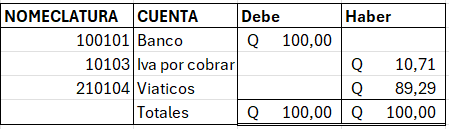
\includegraphics[width=0.8\textwidth]{imagenes/image5.png}
    
    \vspace{0.2cm}
    \raggedright \small \textbf{Nota.} \textit{Tomar en cuenta que las partidas contables contienen su número en la nomenclatura y su nombre.}
\end{figure}

El sistema propuesto desea realizar estas partidas contables de tal manera que el contador, solo ingrese los datos de la factura e indique si contiene algún impuesto, para que estas cuentas se puedan clasifiquen y realicen los cálculos correspondientes de forma automática.

\subsubsection{Optimización de Procesos mediante Alertas y Notificaciones}

La implementación de un sistema de alertas no es solo una funcionalidad técnica, sino una estrategia de control preventivo. Según Estupiñán Gaitán (2015, p. 88), las actividades de control deben incluir mecanismos que aseguren el cumplimiento de las normas y políticas establecidas por la gerencia. En un entorno donde se manejan múltiples obligaciones financieras, la notificación proactiva sustituye a la revisión reactiva, reduciendo drásticamente el margen de error humano.

\textbf{Mitigación del Riesgo de Extemporaneidad.} Uno de los problemas identificados en la empresa, es el retraso en el pago a proveedores debido a fallas en el seguimiento manual. Las alertas automatizadas permiten cumplir con el objetivo contable de "proyectar flujos de caja" y anticipar las salidas de efectivo. Al parametrizar los días de crédito (por ejemplo, 45 días), el sistema garantiza que la administración tenga visibilidad del compromiso antes de que este se convierta en una mora.

\textbf{Gestión de Excepciones y Días Inhábiles.} La lógica del sistema propuesto aborda una debilidad del control manual: la consideración de feriados y fines de semana. En Guatemala, el depósito de cheques posfechados o el pago de obligaciones debe ajustarse al calendario laboral para evitar protestos o recargos.

\begin{itemize}
    \item \textbf{Control de Cheques:} El sistema dará aviso el día correspondiente de depósito, dejando un registro para consultas futuras.
    \item \textbf{Ajuste Automático:} Si una fecha de depósito coincide con un día de descanso, el sistema alerta para realizarlo al siguiente día laboral.
\end{itemize}

\begin{table}[h]
    \centering
    \caption{Jerarquía de Alertas y su Impacto en el Control Interno}
    \vspace{0.2cm}
    \begin{tabular}{p{3cm} p{5cm} p{5cm}}
        \toprule
        \textbf{Tipo de Alerta} & \textbf{Evento Disparador} & \textbf{Objetivo de Control} \\
        \midrule
        Preventiva & 1 día antes del vencimiento de factura. & Asegurar liquidez y solvencia. \\
        Informativa & Registro exitoso de viáticos por colaborador. & Comunicación fluida Contador-Admin. \\
        Crítica & Fecha de depósito de cheque posfechado. & Proteger activos y evitar pérdidas. \\
        Cumplimiento & Límite de gasto en fondo de caja chica. & Promover eficiencia operativa. \\
        \bottomrule
    \end{tabular}
\end{table}

\subsubsection{Sistemas de Información Contable (SIC) y Transformación Digital}

Corresponde al ecosistema donde vivirá el software. Un SIC no es solo una base de datos; es una estructura que combina recursos humanos, tecnológicos y registros para producir información útil.

"Un sistema de información contable recolecta, procesa y comunica información financiera sobre una entidad económica a una amplia variedad de personas" (Meigs et al., 2000, p. 8).

Para la empresa en la cual se desplegará el sistema propuesto, esto representaría la evolución del sistema manual a uno automatizado. Según Estupiñán Gaitán (2015, p. 88),'' la automatización elimina los "cuellos de botella" que se forman cuando la información depende de procesos humanos repetitivos, como la transcripción de datos de facturas a hojas de cálculo''. El contador dejara de utilizar documentos en papel, así como hojas de Excel para realizar todo automatizado por medio del sistema propuesto.

\subsubsection{El Concepto de Computación en la Nube y Repositorios Digitales}

Representan la evolución moderna del almacenamiento y la gestión de la información, por medio de estructuras virtuales que se manejan en torno a la Red de internet, permitiendo así a las organizaciones y/o usuarios poder acceder a esta desde cualquier parte, solamente se necesita algún dispositivo electrónico inteligente, como: Teléfonos móviles, Computadoras. También permite que el almacenamiento crezca conforme la empresa lo requiera, por lo que, la empresa tiene control sobre el mismo.

\subsubsection{Seguridad de la Información y Perfiles de Usuario}

Las organizaciones evalúan riesgos y por medio de este análisis aplican medidas de seguridad de datos tanto para el personal como para la empresa, en el cumplimiento de datos personales. Lo primordial es utilizar contraseñas las cuales deben ser complejas y únicas. Para ello sirve la seguridad de la información, para proteger datos confidenciales mediante políticas y herramientas que garantizan la confidencialidad, integridad y disponibilidad.

Se crean perfiles de usuario, los cuales deben ser por niveles de autoridad, Teniendo como el nivel mas alto. A la persona que puede modificar y administrar la mayoría del software. Esta función mayormente es utilizada para poder limitar el acceso no autorizado y prevención de fugas de información.

"Las actividades de control incluyen verificaciones independientes y la documentación adecuada para asegurar un control efectivo" (Horngren et al., 2012, p. 240). En el sistema propuesto, esto se traduce en la autenticación y Autorización. Definiendo roles con niveles de acceso para poder proteger la información mediante contraseñas y que solo las personas con accesos puedan tener control en ella, algo que en los documentos de Excel no puede garantizar.

\subsection{Marco Tecnológico}

Se hablará sobre las herramientas, lenguajes de programación y metodologías de ingeniería de software que servirán como base para la construcción del sistema propuesto. La sección de estas tecnologías responde a los criterios de seguridad, estabilidad y eficiencia exigidos por el control interno de la empresa don se desplegará el sistema propuesto.

\subsubsection{Metodología de Desarrollo: Proceso Unificado Racional (RUP)}

Se opta por el uso de esta metodología por ser un framework, para el desarrollo de software, estructurado e iterativo, creado por Rational Software (ahora es parte de IBM). Según Sommerville (2011, p. 30), RUP es un modelo de proceso moderno que se caracteriza por ser iterativo e incremental, lo que permite reducir riesgos desde las etapas tempranas del proyecto.

A diferencia de un proceso lineal donde no se ve el resultado hasta el final, RUP permite crear "versiones" pequeñas y funcionales. "El desarrollo iterativo permite que el equipo de desarrollo aprenda de las versiones anteriores y refine los requisitos del usuario" (Sommerville, 2011, p. 30). y organiza el trabajo en cuatro fases criticas:

\textbf{Inicio (Inception).} Se define el alcance del proyecto, visión y se identifican los riesgos principales. Por ejemplo, definimos como un posible riesgo la transición de archivos de Excel a una base de datos centralizada.

\textbf{Elaboración (Elaboration).} Diseña la arquitectura, refina requisitos y mitiga riesgos. Siguiendo el ejemplo anterior, podemos crear las bases de datos para que estas se adapten a la información del Excel.

\textbf{Construcción (Construction)}. Es la fase de programación y diseño de los módulos, también acá se realizan pruebas. Por ejemplo, creamos módulos por cada tipo de función que deseamos como lo podría ser, (Viáticos, Cheques, Caja Chica).

\textbf{Transición (Transition).} El sistema se entrega a los usuarios finales (Contador y Administrador) para pruebas y despliegue. Se realizan capacitaciones para dar a conocer el producto final y resolución de dudas, acá es donde ya se instala el sistema.

"RUP se basa en el uso de casos de uso para guiar el desarrollo y se centra en la arquitectura, lo que garantiza que el sistema sea robusto antes de añadir grandes cantidades de código" (Larman, 2004, p. 25). Casos de Uso: en esencia es como el usuario interactúa con el sistema, el usuario desea realizar una acción como lo es registrar una factura, entonces le debe dar esa indicación al sistema, ingresando los datos de la factura y luego el sistema debe llegar a su objetivo, por ejemplo, el registro de la factura.

\begin{figure}[h]
    \caption{Ejemplo de caso de Uso}
    \vspace{0.2cm}
    \centering
    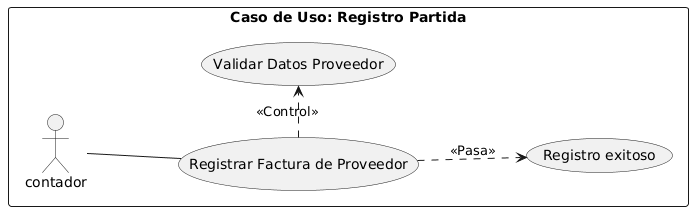
\includegraphics[width=0.8\textwidth]{imagenes/image6.png}
\end{figure}

El ejemplo de la figura 5 demuestra como el contador registra la factura del proveedor, luego el sistema valida los datos del proveedor, para su control y después pasa a su objetivo el cual es el registro exitoso.

\subsubsection{Lenguajes y Herramientas}

\textbf{Angular.} Es la cara del sistema (Frontend). Es decir que es lo que el usuario ve y con lo que interactúa en su pantalla. Angular es un marco de trabajo (framework), el cual fue desarrollado por Google que permite que una página Web tenga la misma sensación como lo es utilizar aplicaciones de escritorio, de manera rápida y fluida.

"Los marcos de trabajo como Angular permiten que el desarrollador se concentre en la experiencia del usuario, automatizando tareas repetitivas de actualización de la pantalla" (Freeman, 2020, p. 45).

"Angular es una plataforma de desarrollo, construida sobre TypeScript. Como plataforma, Angular incluye un marco de trabajo basado en componentes para construir aplicaciones web escalables y una colección de bibliotecas bien integradas que cubren diversas funciones como el enrutamiento y la gestión de formularios" (Google, 2024a, párr. 2).

Esto significa que Angular actúa como un "kit de construcción" profesional que ya tiene todas las piezas seguras para crear modulos se adaptan a cualquier pantalla de computadora.

Esto en el sistema propuesto corresponde a todo el apartado visual e interactivo que vera el usuario.

\textbf{Python.} Es la parte invisible para el usuario (Backend). Es el lenguaje de programación que utilizaremos para la construcción de la lógica de todo el sistema propuesto, desde operaciones básicas, como la automatización de partidas de diario. Se podría decir que es el cerebro de todo el sistema.

"Python destaca por su capacidad para manejar lógica de negocio compleja y su facilidad para integrarse con otros sistemas" (Van Rossum, 2018).

"Python es un lenguaje de programación interpretado, orientado a objetos y de alto nivel con semántica dinámica. Sus estructuras de datos integradas, combinadas con el tipado y el enlace dinámicos, lo hacen muy atractivo para el desarrollo rápido de aplicaciones" (Python Software Foundation, 2024, párr. 1).

En términos sencillos esto significa que Python permite escribir las reglas de negocio (como el cálculo de impuestos guatemaltecos o alertas de cheques) de forma clara y segura, facilitando que el sistema sea fácil de mantener y actualizar en el futuro.

Se opta por Python por su gran versatilidad, por lo que se permite usarse en casi cualquier campo tecnológico. Su sintaxis es sencilla, contiene una amplia selección de librerías, su comunidad es inmensa y no utiliza tantas líneas de código como otros lenguajes de programación.

\textbf{PostgreSQL}, Es una base de datos gratuita y potente, Usa el lenguaje de SQL y esta preparado para maneja de forma segura la información.Al ser de codigo abierto tiene tuna gran comunidad de programadores en todo el mundo, por lo que se mantiene actualizada y con mejoras constantes.

"PostgreSQL incluye numerosas funciones diseñadas para ayudar a los desarrolladores a crear aplicaciones, a los administradores a proteger la integridad de los datos y crear entornos tolerantes a fallos, y a gestionar sus datos independientemente de su tamaño. Además de ser gratuito y de código abierto , PostgreSQL es altamente extensible. Por ejemplo, puede definir sus propios tipos de datos, crear funciones personalizadas e incluso escribir código en diferentes lenguajes de programación sin necesidad de recompilar la base de datos" (PostgreSQL Global Development Group, s. f., párr. 1).

\textbf{Token JWT}. Sirve como metodo de seguridad que al momento de que un usuario desea ingresar debe verificar si este existe en la base de datos PostgreSQL, a partir de ello pasa por el backend quien valida que tipo de accesos tiene y estos se muestran en el Angular al abrir el navegador

Si el contador registra un cheque desde su oficina, el administrador verá la actualización en su pantalla instantáneamente sin necesidad de refrescar la página o enviar archivos por correo electrónico.

"PostgreSQL admite varios métodos de autenticación de clientes. Cuando un cliente se conecta al servidor de base de datos, especifica con qué nombre de usuario de base de datos desea conectarse. Luego, el servidor determina si acepta la conexión en función del método de autenticación configurado para ese cliente y usuario." (PostgreSQL Global Development Group, 2024, cap. 21).

"El módulo pgcrypto proporciona funciones criptográficas para PostgreSQL. Incluye funciones para el almacenamiento con resumen cifrado de contraseñas (hashing), cifrado de clave simétrica y cifrado de clave pública."(PostgreSQL Global Development Group, 2024, apendice F).

\begin{table}[htbp]
    \centering
    \caption{Analogía y Comparación entre el Sistema Actual y el Propuesto}
    \label{tab:comparativa_sistema}
    \vspace{0.2cm}
    \begin{tabular}{p{3cm} p{5.5cm} p{6.5cm}}
        \toprule
        \textbf{Concepto} & \textbf{Sistema Actual (Manual/Excel)} & \textbf{Sistema Propuesto (Web)} \\
        \midrule
        \textbf{Almacenamiento} & Archivos en disco duro local u hojas de cálculo aisladas. & Base de datos relacional PostgreSQL con acceso centralizado. \\
        \addlinespace
        \textbf{Seguridad} & Sin restricciones o archivos protegidos con clave simple; cualquiera puede editar. & Autenticación por tokens (JWT), control de roles y permisos por usuario. \\
        \addlinespace
        \textbf{Cálculos e Integridad} & Fórmulas en Excel susceptibles a borrado o modificación accidental. & Lógica de negocio automatizada en Python con validación en Angular. \\
        \addlinespace
        \textbf{Respaldos} & Copias manuales esporádicas en memorias USB o correos electrónicos. & Respaldos automatizados (\textit{backups}) e integridad transaccional ACID. \\
        \bottomrule
    \end{tabular}
\end{table}